%------------------------------------------------------------------
%	TEMPLATE INFORMATION
% This template has been downloaded from:
% http://www.LaTeXTemplates.com

% Original author:
% Frits Wenneker (http://www.howtotex.com) with extensive modifications by Vel (vel@LaTeXTemplates.com)

% License:
% CC BY-NC-SA 3.0 (http://creativecommons.org/licenses/by-nc-sa/3.0/)


%------------------------------------------------------------------
%	PACKAGES AND OTHER DOCUMENT CONFIGURATIONS
\documentclass[twoside,twocolumn]{article}
\linespread{1.03} % Line spacing

\usepackage{blindtext} % Package generate dummy text
\usepackage{textcomp}
\usepackage{lipsum}
\newenvironment{Figure}
  {\par\medskip\noindent\minipage{\linewidth}}
  {\endminipage\par\medskip}
\usepackage{graphicx}
\usepackage[sc]{mathpazo} % Use the Palatino font
\usepackage[T1]{fontenc} % Use 8-bit encoding
\usepackage{microtype} % Slightly tweak font spacing
\usepackage[english]{babel} % Language hyphenation
\usepackage[hmarginratio=1:1,top=26mm, bottom=26mm, left=2cm, right=2cm, columnsep=20pt]{geometry}
\usepackage[hang, small,labelfont=bf,up,textfont=it,up]{caption}
\usepackage{booktabs} % Horizontal rules in tables
\usepackage{enumitem} % Customized lists
\setlist[itemize]{noitemsep} % Make itemize lists more compact
\usepackage{mathabx}

\usepackage{abstract} % Allows abstract customization
\renewcommand{\abstractnamefont}{\normalfont\bfseries}
\renewcommand{\abstracttextfont}{\normalfont\small\itshape}

\usepackage{titlesec} % Allows customization of titles
\renewcommand\thesection{\Roman{section}}
\renewcommand\thesubsection{\Roman{section}.\roman{subsection}}
\renewcommand\thesubsubsection{\Roman{section}.\roman{subsection}.\roman{subsubsection}}
\titleformat{\section}{\large\scshape\bf}{\thesection}{1em}{\MakeUppercase} 
\titleformat{\subsection}[block]{\large\bf}{\thesubsection}{1em}{}
\titleformat{\subsubsection}[block]{\large\it}{\thesubsubsection}{1em}{}

\usepackage[export]{adjustbox}
\usepackage{fancyhdr} % Headers and footers
\pagestyle{fancy} % All pages have headers and footers
\fancyhead{$\bullet$------------------------------------------$\bullet$} %fancy header
\fancyhead[c]{Comparative Analysis for NLP $\bullet$ Aug. 2017}
\fancyhead[r]{$\bullet$----------------------------------------$\bullet$ \thepage}
\lfoot{
\includegraphics[scale=0.12,valign=c]{ORNL_Logo.png}}
\cfoot{
\includegraphics[scale=0.072,valign=c]{ORISE_Logo.png}}
\rfoot{
\includegraphics[scale=0.08,valign=c]{DOE_Logo.png}}

\usepackage{titling} % Customizing the title section
\usepackage{hyperref} % For hyperlinks in the PDF
\usepackage{apacite}


%------------------------------------------------------------------
%	TITLE SECTION
\setlength{\droptitle}{-4\baselineskip} % Move the title up
\pretitle{\begin{center}\large\bfseries} % Article title formatting
\posttitle{\end{center}} % Article title closing formatting
\title{Comparative Analysis of Text Representation Embeddings for\\ Natural Language Processing} % Article title
\author{
 Jonathan, Gibson A.\\ 
  \texttt{Tennessee Tech University}\\
  \texttt{jagibson44@students.tntech.edu}
  \and
  Dr. Christian, James B.\\
  \texttt{Oak Ridge National Laboratory}\\
  \texttt{christianjb@ornl.gov}
}
\date{\today}
\renewcommand{\maketitlehookd}{
\begin{abstract}
\noindent 
Natural Language Processing (NLP) is a vast, powerful field capable of complex textual analysis. However, identifying the optimal method for analyzing any unique text set is a challenge. Further, preprocessing techniques change with an embedding\textquotesingle s purpose and impose additional complications. We compared and identified strengths and weaknesses of two word-embedding models for document classification: Graph of Words (GoWs) and n-Grams. GoWs rely heavily on relative proximity of terms in sequence, while n-grams create embeddings based on strict, original word order. Unfortunately, both models tend to provide many ineffective or semantically similar features from the documents they analyze. GoWs and n-grams have similar problems, yet GoWs generally seem more resilient. For this reason, we suspected that a robust GoWs model might perform better than traditional n-gram models, given the same parameters. The National Cancer Institute (NCI) requires that cancer pathology report data be entered into a structured database containing basic tumor information. These reports contain censored, confidential patient information and specifics regarding size, code, stage, location, and histological grade of tumors, in plain text. We sought to find the best word-embedding method for analyzing approximately 250,000 such reports. There is no standard approach for writing these reports and many are not explicitly labeled with an ICD-O-3 topographical code specifying the tumor\textquotesingle s anatomical site of origin. This deficit decreases the size of the training data set and moderately reduces predictive power. Although these reports were not designed for external algorithmic analysis, NLP allows us to automate the extraction of important terms for uses such as treatment outcomes and recurrence relations. Given the same parameters, the GoWs classification accuracy was almost equivalent to that of the n-grams, but noticeably decreased with increased window size.
\end{abstract}
}

\begin{document}
% Print the title
\maketitle
\thispagestyle{empty}


%------------------------------------------------------------------
%	CATEGORIES AND SUBJECT DESCRIPTORS
\section*{Categories and Subject \\Descriptors}

E.1 [\textbf{Data}]: Data Structures - Graphs and Networks;
I.2.7 [\textbf{Artificial Intelligence}]: Natural Language Processing;
I.7.0 [\textbf{Document and Text Processing}]: General;


%------------------------------------------------------------------
%	KEYWORDS
\section*{Keywords}
graph of words; n-grams; NLP; natural language processing; comparative analysis; word embeddings; cancer;


%------------------------------------------------------------------
%	ARTICLE CONTENTS
%	SECTION: INTRODUCTION
\section{Introduction}
In the United States, cancer mortality and incidence rates have been slowly declining, as of 2014, \cite{nci_2014} due to new medical advances and techniques for treating tumors. However, this fact does not reduce the severity and importance of working towards a cure for cancer. In the year 2016 alone, $\approx$1.7 million people suffered and $\approx$600,000 people died from cancerous tumors \cite{nci_2017}.\\
\\
When any patient has a surgery, is diagnosed with a disease, or simply goes to a clinic for a check-up, doctors and medical professionals make detailed records of these occurrences; it is no different when dealing with cancer records. There are databases that contain a slew of detailed cancer pathology reports specifying all kinds of tumor, patient, and treatment information. The quantity of data held within these databases is just kind that is useful for machine learning (ML) \& NLP algorithms: large learning corpuses. Although not originally designed for ML or NLP analysis, sophisticated pathology report analytic algorithms could be a small piece in the cancer curing puzzle. The introduction of such an automated ML or NLP analysis and recording system could provide doctors and medical professionals time to focus on patient care and beneficial cancer research.\\
\\
The rest of this paper is organized as follows. In section 2 we examine the finer problem details within the pathology reports. In section 3 we discuss the NLP models and methods used to arrive at our results and the complications associated with them. Section 4 reveals such results. We summarize our findings in section 5. Finally, section 6 defines other implementations that could be added to our models, potentially for improved performance.


%------------------------------------------------------------------
%	SECTION: PROBLEM DEFINITION

\section{Problem Definition}
Cancer pathology reports exist in incredibly large quantities and require robust autonomous algorithms to efficiently extract useful information. The NCI\textquotesingle s Surveillance Epidemiology and End Results (\textit{SEER}) program, among others, house large data bases of such reports. These reports were originally designed to stay within the medical field and only be used by M.D.'s and pathologists; recently they\textquotesingle ve been used for secondary purposes, such as ML \& NLP analysis. We have been tasked to find a plausible, efficient, and accurate method of evaluating $\approx$256,000 reports (\textit{of which only $\approx$20,000 are labeled with ICD-O-3 topographical codes}) for purposes such as topographical code classification, treatment outcomes, and recurrence relations. However, we currently only have access to 2505 reports (\textit{of which only 942 are labeled with ICD-O-3 topographical codes}). In our experiments, we dealt with topographical code classification exclusively. \textbf{Table 1} outlines the categories, iterations, and definitions of the topographically labeled reports. If a particular report does not contain information about the specific location of a tumor within its respective organ, it is marked as: Not Otherwise Specified (\textit{NOS}). \textbf{Table 2} shows which registries (Connecticut, Kentucky, Hawaii, Seattle, and New Mexico) contributed to the topographically labeled reports that we used in our experiments.

\begin{table}
\caption{ICD-O-3 Topographical Codes}
\centering
\resizebox{0.45\textwidth}{!}{%
  \begin{tabular}{lll}
  \toprule
  Code & Count & Description\\
  \midrule
  C34.0 & 26 & Main Bronchus\\
  C34.1 & 139 & Lung, Upper Lobe\\
  C34.2 & 11 & Lung, Middle Lobe\\
  C34.3 & 78 & Lung, Lower Lobe\\
  C34.9 & 191 & Lung, NOS\\
  C50.1 & 13 & Breast, Central Portion\\
  C50.2 & 36 & Breast, Upper-Inner Quadrant\\
  C50.3 & 10 & Breast, Lower-Inner Quadrant\\
  C50.4 & 63 & Breast, Upper-Outer Quadrant\\
  C50.5 & 21 & Breast, Lower-Outer Quadrant\\
  C50.8 & 62 & Breast, Overlapping Lesion\\
  C50.9 & 292 & Breast, NOS\\
  \bottomrule
  \end{tabular}%
}
\end{table}


\begin{table}
\caption{Labeled Pathology Report Contributions}
\centering
\resizebox{0.3\textwidth}{!}{%
	\begin{tabular}{lll}
	\toprule
    Registry & Lung & Breast\\
    \midrule
    CT & 32 & 44\\
    KY & 105 & 96\\
    HI & 102 & 109\\
    Seattle & 93 & 117\\
    NM & 113 & 131\\
    \bottomrule
	\end{tabular}
}
\end{table}

\subsection{Tokenization}
Because these pathology reports hold confidential information about doctors and their patients, the reports contain a set of variables (\textit{tokens}) that conceal this sensitive/personal information from us. These tokens include but are not limited to: **INITIALS, **DATE, **FLOATTOKEN, and **NAMETOKEN. These tokens are preceded by asterisks to indicated the start of a confidential variable. 

\subsection{Pathology Report Inconsistencies}
Throughout all of the pathology reports, there is not a standard way to represent tokens, abbreviations, or abbreviated phrases (\textit{**NAMETOKEN vs. *nametoken, Dr. vs. dr., o'clock vs. O'clock, P.M. vs. PM, A.M. vs. AM, etc...}). Although sensible for human eyes, these simple inconsistencies are problematic for ML \& NLP analysis. Any ML or NLP model that doesn\textquotesingle t account for these inconsistencies will recognize different abbreviations or tokens as separate inputs, when in reality they have the same meaning. In subsubsection \textit{III.i.iv} we will address how we dealt with this particular problem.\\
\\
Not only are there syntactical inconsistencies in these reports, but there are also inconsistencies regarding the overall structure. Some of the reports are structured as paragraphs while others are structured as bulleted notes or with organized sections and subsections. There are also differences in the lengths of the reports. Although the structural differences may not negatively effect our model, the length of each report could determine the model's ability to learn from the respective report's class.

\subsection{Insufficient Labeling}
For the purpose of analyzing data of any kind using ML or NLP analysis, it is important to have enough data for your model to learn from in order to provide sufficient output(s). When a model is given enough data, the model has a larger training set, contributing to more accurate predictions. Inversely, when a model is given an insufficient amount of data, the model makes worse predictions based on the limited training set. In the case of our available corpus, there is a large margin of variability regarding the iterative number of each topographical category/class. Looking at the numbers from \textbf{Table 1} you can see that classes C34.1, C34.9, and C50.9 account for $\approx$66\% (\textit{622/942}) of our experimental data. Based on the number of available pathology reports, all the other classes fall short of the appropriate count necessary ($\lessapprox$ \textit{100 iterations}) for sufficient classification accuracy. \textbf{Figure 1} gives a color coded representation of sufficiency in our topographical labeling. Other than providing more data by collection or augmentation, there is not a clear, easy way to fix this problem.

\begin{Figure}
 \centering
 \label{fig:bar}
 \captionof{figure}{Rating of classes based on topographical label iterations.}
 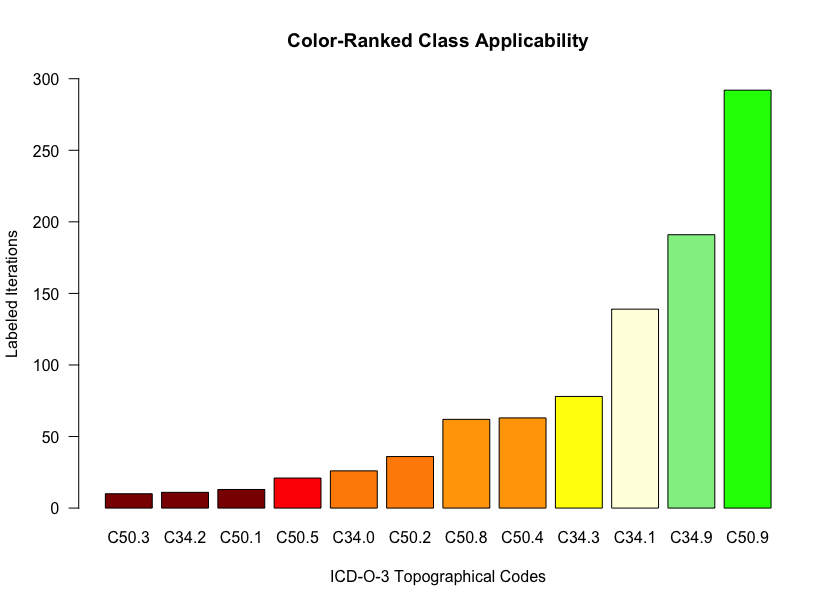
\includegraphics[width=\linewidth]{Barplot_Final.png}
\end{Figure}


%------------------------------------------------------------------
%	SECTION: METHODS
\section{Models \& Methods}

The models and methods that we implemented to achieve our results are as follows: 
\begin{itemize}
\item \textbf{Preprocessing}
	\begin{itemize}
	\item Punctuation Removal
    \item Stopword Removal
    \item Stemming
    \item Inconsistent Text Cleaning
	\end{itemize}
\item \textbf{Graph of Words}
	\begin{itemize}
    \item Supergraphs
	\item Subgraphs
    \item Induced Subgraphs
    \item Window Size
	\end{itemize}
\item \textbf{n-Grams}
	\begin{itemize}
	\item Bag of n-Grams
	\end{itemize}
\item \textbf{Random Forest Classification}
	\begin{itemize}
	\item Decision Trees
	\end{itemize}
\item \textbf{Support Vector Machine Classification}
	\begin{itemize}
	\item Hyperplanes
	\end{itemize}
\end{itemize}

If you are familiar with all of these models and methods, skip to section \textbf{IV} (\textit{pg. 5}) for the results.

\subsection{Preprocessing}
Preprocessing is an essential step for many ML \& NLP models. It is the process of taking formatted data and turning it into raw usable input for your desired model. Preprocessing steps will change based on your corpus, your purpose, and your chosen model. Although one of the more simpler steps in a ML or NLP algorithm, preprocessing decisions can effect your model's eventual performance.

\subsubsection{Punctuation Removal}
This is the most basic step of any text preprocessing. After the removal of all punctuation/special characters from the text, the text is much easier to parse. Without the removal of punctuation, the model's output would be cluttered with symbols instead of words or characters. Some researchers have left periods in the text as to not associate the ending word of one sentence with the beginning word of the next sentence \cite{Markov:2006:FCW:1784815.1784819}; we did not implement that specific function in our experiments. For our experiments we simply removed all punctuation and special characters.

\subsubsection{Stopword Removal}
Another basic step of text preprocessing is the concept of stopword removal. Stopwords are words in a text that provide little to no meaning for the theme of the document and occur far too frequently to count their contribution. When stopwords are not taken out of data before input, the model is overrun by insignificant words that clutter the output and its ability to make proper predictions. We used the English stopword list from the NLTK library; it includes words like: it, am, if, an, and most prepositions. This tactic is very common in the fields of ML \& NLP because it is easy to implement and can help make improvements to many models \cite{rousseau2015text}.

\subsubsection{Stemming}
A slightly more complicated step of preprocessing is the action of stemming. Due to some of the complications within the English language, there exist words that have the same root and meaning but would be taken as different words by most ML \& NLP models. Imagine the words: compute, computed, computes, computing, and computer. All 5 of these words have the same relative meaning, but since they are not spelled the same, they would be counted as different words if not stemmed. When stemmed, these 5 words are reduced to a single root word: "comput". This allows all iterations of similar meaning to be combined into one root word. This process is repeated for all other equivalently rooted words. Again, without the addition of the stemming process, a model's output would be cluttered with unnecessary words. We used the NLTK Porter Stemmer for our purposes \cite{Markov:2006:FCW:1784815.1784819}.

\subsubsection{Inconsistent Text Cleaning}
Although this step was a bit more specific to our corpus, similar actions could be taken to improve the performance of other ML \& NLP models. We mentioned in subsection \textbf{II.iii} that there were inconsistencies with some terms such as: variable tokens, Dr., o'clock, P.M., A.M., etc..., but with text cleaning we intend to find all of those inconsistencies and change each one to a consistent version of itself. For example, there are many different ways to abbreviate the phrase "post meridiem" (\textit{PM, P.M., pm, p.m., P.m., etc...}) but we changed all possible iterations of this abbreviation to "pm" specifically. This is yet another example of a preprocessing step that will help avoid cluttering a model's output with useless information.\\
\\
After this process, we created a list of individually parsed words as raw input data. We then fed the list of words into either a GoWs model or an n-gram model. Each model created a different set of extracted features that we later used for predictive input into a Support Vector Machine (SVM) and Random Forest (RF) classifier.

\subsection{Graph of Words}
The graph of words word embedding model is simple, yet effective. It takes advantage of relative structure of text rather than specific ordering of words. Unique words in a document are presented as vertecies and words within a certain \textbf{window size} of proximity are connected and presented as edges. For our purposes, each pathology report was analyzed by the GoWs model and structured as a separate \textbf{supergraph}. These supergraphs were then mined to reveal every possible \textbf{subgraph}. These subgraphs are simply subsets of their respective parent supergraph and are the potential predictive features for the model. In order for a subgraph to be worthy of becoming a feature for the model, it must occur in separate supergraphs at least as frequently as the minimum \textbf{support value}. We assigned 1 as the minimum vertecies value and 5 as the maximum vertecies value for our feature subgraphs. Our support value required that the features occur in at least 10\% of the available corpus. After the subgraph features have been selected, their information is then converted into mathematical feature vectors for SVM and RF classification input.

\begin{Figure}
 \centering
 \label{fig:subgraph}
 \captionof{figure}{A sample subgraph from a cancer pathology report officially labeled as right breast cancer (window size = 4).}
 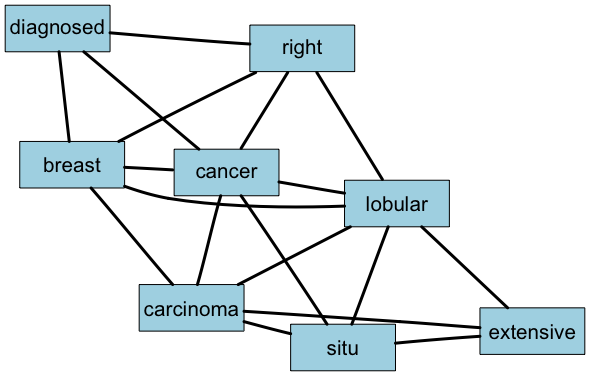
\includegraphics[width=\linewidth]{Rgraphviz_Subgraph.png}
\end{Figure}

\subsubsection{Induced Subgraphs}
The Encyclopedia of Mathematics defines induced subgraphs as the following:\\
\\
Given a subgraph \textit{G}:\\
An induced subgraph is the graph \textit{G[S]} having \\
(1) As a given vertex subset \textit{S}, the vertex set of \textit{G};\\
(2) Edges between \textit{x,y} $\in$ \textit{S};\\
(3) All edges that exist between \textit{x,y} in \textit{G}.\\
\cite{mathematics_2016}\\
\\
In other words, given any subgraph, if a separate subgraph is created from a different context but contains the exact same connections, the subgraphs are functionally equivalent and therefore, induced subgraphs. Our GoWs model algorithm omitted induced subgraphs from the potential subgraph feature list. The removal of these induced subgraph features helps to eliminate feature redundancy prior to classification. It also helped to focus the training set on the most important features, rather than feeding the classification models useless information. As is with any many ML \& NLP learning algorithms, useful/important features increase model performance while useless/un-important features could "confuse" the model and decrease performance.

\subsection{n-Grams}
The n-gram word embedding model is also a simple, yet effective method. It takes advantage of specific ordering of words rather that relative structure of text. All words in each document are placed in separately parsed lists with the length of each list determined by the minimum and maximum word count values. After the creation of these parsed lists, they are collected into a \textbf{bag of n-grams} (\textit{a collection of the model\textquotesingle s extracted features}). During our experiments, we used the n-gram model as a based line to judge the relative changes of the GoWs model. We assigned 1 as the minimum word count value and 5 as the maximum word count value for our n-gram features. Our support value required that the features occur in at least 10\% of the available corpus. Like the GoWs model, these features are then converted into mathematical feature vectors for SVM and RF classification input.

\subsection{RF Classification}
After the extraction of features that are deemed worthy to be predictors, by the GoWs and n-gram models respectively, we used these features as input for RF classification. RF classification uses majority vote \textbf{decision trees} to decide how to classify a particular piece of information. Whichever class is chosen by the majority of the decision trees is the assigned class for any respective prediction. \textbf{Figure 3} shows a generalized form of multiple decision trees \cite{srivastava_shaikh_jain_gupta_gupta_2015}. Generally speaking, when you have many (\textit{decision}) trees, you get a (\textit{random}) forest.

\subsection{SVM Classification}
Using the same features that we used for the RF classification, we also used them as input for SVM classification. SVMs and RFs classify input differently and can yield different accuracy outputs despite similar inputs. Research has shown that SVMs scale well, work well with large data sets \cite{basu2003support}, and eliminate the need for extensive parameter tuning \cite{joachims1998text}. \textbf{Figure 4} shows an example of a binary, linear SVM classifier \cite{sforza_lippi_2013}. The algorithm finds the optimal \textbf{hyperplane} with the largest distance between the closest observations from each class. The lines that are formed parallel to this center margin are called the support vectors.

\begin{Figure}
 \centering
 \label{fig:RFC_Ex}
 \captionof{figure}{A simple example of how random forests use decision trees and majority voting as a basis for classification.}
 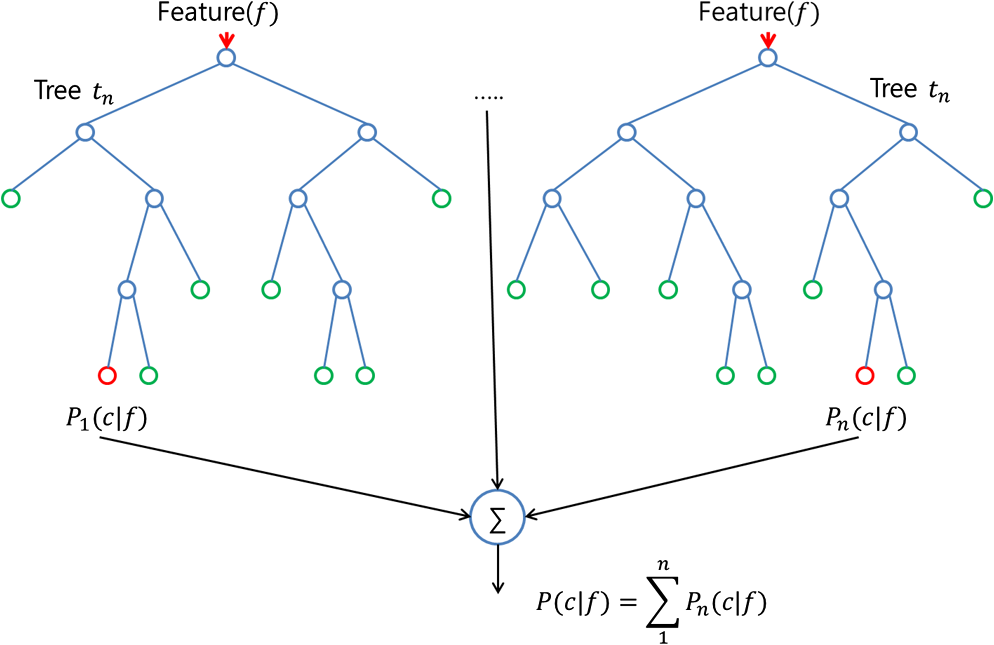
\includegraphics[width=0.8\linewidth]{RFC_Ex.png}
\end{Figure}

\begin{Figure}
 \centering
 \label{fig:SVM_Ex}
 \captionof{figure}{A simple example of linear binary classification using an optimal hyperplane and its support vectors.}
 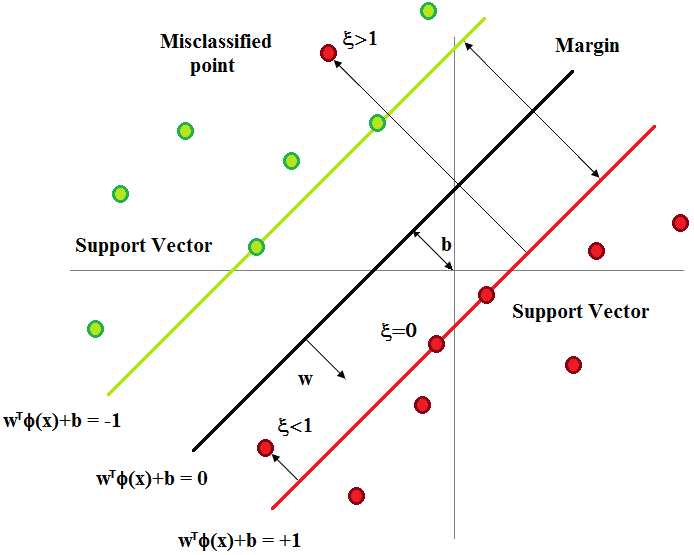
\includegraphics[width=\linewidth]{SVM_Ex.png}
\end{Figure}


%------------------------------------------------------------------
%	SECTION: RESULTS

\begin{figure*}
  \caption{With the n-gram model as a baseline, the number of extracted features as the sliding window size for the GoWs model varies.}
  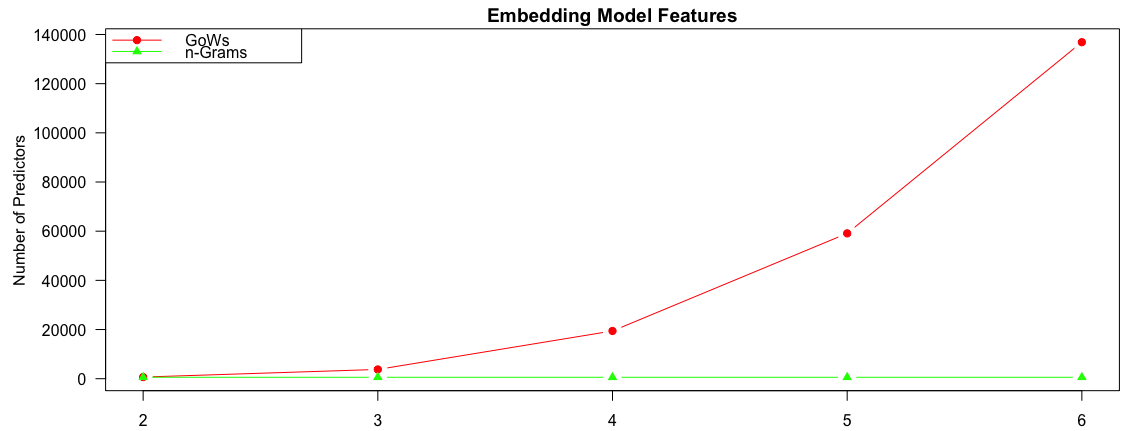
\includegraphics[width=\textwidth,height=6cm]{Feature_Results.png}
\end{figure*}

\begin{figure*}
  \caption{With the n-gram model as a baseline, the relative SVM accuracy as the sliding window size for the GoWs model varies.}
  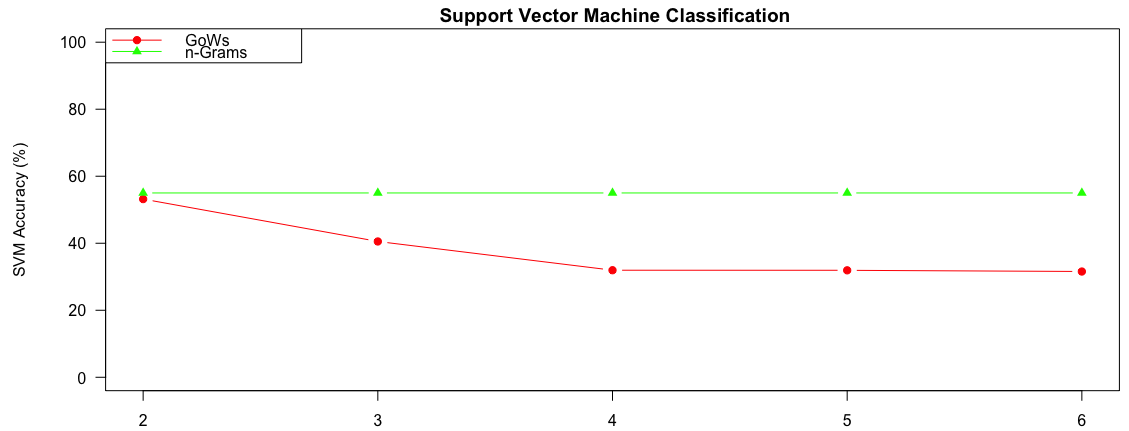
\includegraphics[width=\textwidth,height=6cm]{SVM_Results.png}
\end{figure*}

\begin{figure*}
  \caption{With the n-gram model as a baseline, the relative RF accuracy as the sliding window size for the GoWs model varies.}
  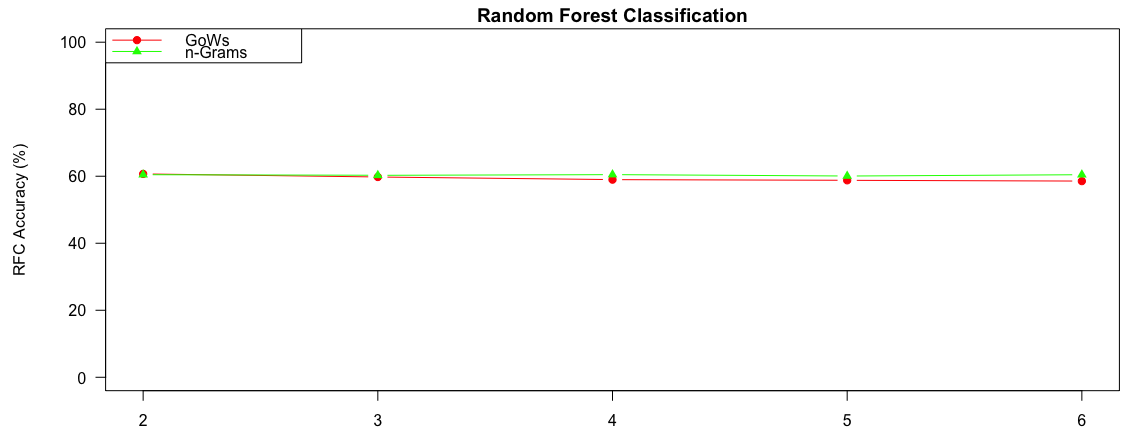
\includegraphics[width=\textwidth,height=6cm]{RFC_Results.png}
\end{figure*}

\section{Results}
As the window size increased for the GoWs model, the number of features increased significantly; this result was expected. However, as the number of features increased, the SVM and RF classification accuracy decreased. The SVM classification accuracy decreased with a much steeper margin. These results are displayed in \textbf{Figures 5, 6, \& 7}. Seeing better performance with smaller feature sets rather than larger feature sets is consistent with \cite{basu2003support}. In order to maximize classification accuracy we must limit the amount of predictive features being produced. But, aggressive feature selection can lead to loss of information and, ultimately, performance loss \cite{joachims1998text}. Less variation in the distribution of available labeled reports will improve performance for both models and for both classification algorithms. In general, well populated classes lead to superior performance while insufficiently populated classes lead to inferior performance.



%------------------------------------------------------------------
%	SECTION: CONCLUSION
\section{Conclusion}
In this paper we stressed the necessity of cancer research, defined the problems with autonomous information extraction from cancer pathology reports, defined 2 NLP word embedding models and 2 classification algorithms for analyzing such reports, and outlined the results of our comparative analysis between GoWs and n-grams. Even though the classification accuracy of the GoWs model decreased in both SVM and RF classification, we are confident that the GoWs model could significantly out-perform the n-gram model if some, or all, of the functions from subsection \textbf{VI.i} were implemented. Based on our results, we suspect that the predictive capabilities for cancer pathology reports may rely more on word order rather than relative word structure. 


%------------------------------------------------------------------
%	SECTION: ACKNOWLEDGEMENTS
\section{Future Work}
If not already implemented, all of these functions could potentially improve performance of either GoWs or n-gram models.

\subsection{Additional GoWs Options}

\paragraph{GoWs Dropout:} Dropout is a popular and effective tool widely used for Artificial Neural Networks (\textit{ANNs}). Dropout simulates the "deactivation" of an network\textquotesingle s neurons during forward and back propagation. This forces the algorithm to resist over-fitting the training data and potentially perform better during test time. Although we were unable to test our hypothesis, we would like to propose a version of dropout for GoWs models. Suppose you randomly choose 10-50\% of a subgraph's vertices and deleted them before converting the subgraph into its respective feature vector. Similar to traditional Convolutional Neural Network (\textit{CNN}) dropout, this function could help make the GoWs model more robust.

\paragraph{Edge Weights:} Edge weights add a statistic for relative probability, based on currently connected vertices, that any particular word will occur after the word (\textit{vertex}) in question. These weights are directly and linearly correlated to the number of co-occurrences of respective bi-grams (\textit{every 2 word sequence}). The weight values are updated after each of these respective bi-gram throughout the whole document \cite{Rousseau2015}.

\paragraph{Main Core (\textit{k}-Core):} The main core of a supergraph is the maximally connected subgraph whose word vertices occur at least '\textit{k}' times within the supergraph. The number of core terms in any given supergraph should be decided an individual document basis; even for documents of equal length in the same dataset, some cores may need to be larger than others based on respective document content variation \cite{Rousseau2015}. Main cores provide much needed emphasis on phrases that have high probability and strong predictive power. 

\paragraph{Directed Edges:} Directed edges define a particular direction of words in a document, without them, you lose knowledge of the first word in any given bi-gram. This is similar to the default function of n-grams \cite{Markov:2006:FCW:1784815.1784819}.

\paragraph{Edge Labels:} Edge labels define the section of a document or article that any particular word connection originated. These labels can be from titles, text bodies, hyperlinks, etc... (\textit{TI, TX, L, respectively}). This functional addition may not be helpful in our corpus, but can be especially useful for web pages \cite{Schenker03classificationof}.


\subsection{Additional n-Gram Options}

\paragraph{n-Gram Dropout:} Although not yet tested, we would like to propose an n-gram version of dropout. Similar to GoWs dropout, n-gram dropout would delete a certain percentage of randomly selected n-grams before converting them into features for training. Again, this could function could help resist over-fitting creating a more tempered model.

\paragraph{Gram-Weights:} Although not yet tested, we would like to propose an n-gram version of probability weights. Similar to edge weights, gram-weights would keep track of the number of co-occurrences for every unique n-gram. If any particular n-gram has a gram-weight value higher than 1, its relative predictive influence is increased proportionately. This function could help increase the amount of predictive information gathered from any analyzed document.
%------------------------------------------------------------------
%	SECTION: RELATED WORK
\section*{Related Work}
Qui et al. provides a similar analysis of these pathology reports using CNNs and Term Frequency-Inverse Document Frequency (\textit{TF-IDF}). They provide an extensive comparative analysis of these two methods \cite{qiu2017deep}.


%------------------------------------------------------------------
%	SECTION: ACKNOWLEDGEMENTS
\section*{Acknowledgements}
This work was supported in part by the Oak Ridge Institute for Science and Education (\textit{ORISE}), U.S. Department of Energy (\textit{DOE}), Office of Science, and Office of Workforce Development for Teachers and Scientists (\textit{WDTS}) under the Science Undergraduate Laboratory Internship (\textit{SULI}) program.\\
\\
I would also like to thank my mentor \& co-author (\textit{James B. Christian}), and my helpful colleague \& friend (\textit{Michael T. Engen}) for the support, insight, and time that they invested for the betterment of this project.


%------------------------------------------------------------------
%	REFERENCE LIST
\bibliographystyle{apacite}
\bibliography{Full_Bibliography}

\end{document}
